\chapter{GameObject ``Player`` \& Komponenten}

Die Spielfigur, die der Anwender bedient stellte sich w"ahrend der Entwicklung als komplexestes GameObject heraus. In diesem Kapitel geben wir daher einen "Uberblick "uber die Realisierung mithilfe von Sprites sowie der verschiedenen anh"angenden und selbsterstellten Skripte

\begin{figure}
	\centering
	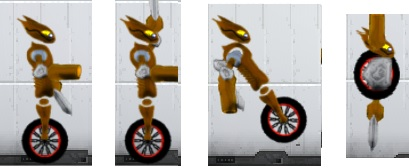
\includegraphics[height=5cm]{images/AnimationenZusammenschnitt.jpg}
	\caption{Zusammenschnitt der Player Sprites}
	\label{fig:playerSprites}
\end{figure}

\section{SpriteRenderer}

\section{AttributeComponent Skript}
Die AttributeComponent dient dazu die spielmechanischen Daten zu hinterlegen und zu verwalten. Sie kann sowohl dem Spieler als auch freundlich und feindlich Gesinnten NPCs angehängt werden. 

Nachfolgend werden die wichtigsten Daten vorgestellt:
\begin{lstlisting}[breaklines=true]
//Lebenspunkte, maximale Lebenspunkte, Ruestung und Schaden
public float health, maxHealth, armor, damage;
//Maximale Ausdauer, Ausdauer und regenerierte Ausdauer pro Sekunde
public float maxStamina, stamina, staminaPerSecond;
//Munition, Munitionskapazitaet und Reichweite
//Range = 0 -> Nahkampf / Range > 0 -> Fernkampf
public int ammo, ammoCap, range;
//Klon aktiv?
public bool cloneAlive = false;

//Cooldown für Plasmaschuss
static float cooldown1 = 1.0f;
//Laeuft cooldown für Plasmaschuss?
bool cooldown1Active = false;

//Cooldown fuer Klonfaehigkeit
static float cooldown2 = 10.0f;
//Time-to-live für Klon
static float ttl = 5.0f;
//Aktuelle Time-To-Live
float attl = ttl;
//Laeuft cooldown fuer Klon?
bool cooldown2Active = false;

//Referenz auf das Nahkampfsystem
MeleeSystem meleeSys;
\end{lstlisting}

Die Update-Funktion der AttributeComponent wird ausschlie"slich dazu benutzt, die Stamina "uber Zeit aufzuf"ullen w"ahrend die fixedUpdate-Funktion für das löschen des Klones verantwortlich ist.
\begin{lstlisting}[breaklines=true]
void Update () {

/*Fuelle Ausdauer ueber Zeit wieder auf solange maximalStamina nicht erreicht ist und die
Spielfigur sich nicht bewegt*/
if (staminaPerSecond > 0.0f && stamina < maxStamina && !meleeSys.animationRunning)
{
//Stelle sicher, dass Stamina nicht kleiner als 0 oder groesser als maximalStamina gesetzt wird
stamina = Mathf.Clamp(stamina+staminaPerSecond * Time.deltaTime,0,maxStamina);
}   
}
void FixedUpdate()
{
if (attl > 0)
attl -= Time.deltaTime;
if (attl <= 0 && cloneAlive)
{
Destroy(GameObject.Find("Klon"));
cloneAlive = false; 
}
}
\end{lstlisting}

\section{CharacterMovement Skript}



\section{MeleeSystem Skript}
Der Nahkampf der Spielers ist wie folgt konzeptioniert:
Dr"uckt ein Spieler die entsprechende Taste, wird ein Schlag ausgef"uhrt. Dr"uckt der Spieler w"ahrend dieser Schlag durchgef"uhrt wird erneut die Schlagtaste, wird eine Folgeschlag eingereiht, welche unmittelbar danach begonnen wird. Somit wird eine Art Nahkampf-Kombo-System umgesetzt, welches bis zu vier Schl"age ausf"uhren kann. Danach wird wieder mit dem ersten Schlag begonnen. Erleidet der Spieler w"ahrend des Kombos einen Treffer, so soll die Kombo abbrechen, und er muss erneut von vorne beginnen.

In diesem Skript arbeiten die Animator Component von Unity eng mit dem MeleeSystem Skript zusammen. Wird der Schlag bet"atigt, wird ein Trigger im Animator ausgel"ost, der die entsprechende Animation aufruft. In dieser Animation wird an einem enstprechenden Keyframe der Schaden durchgef"uhrt, sodass es passend zur Animation stattfindet. W"ahrend die Animation l"auft, ist ein bool'scher Wert so gesetzt, dass neue Schlagaktionen als Kombo interpretiert werden. Ist das der Fall, wechselt der Animator am Ende einer Schlaganimation in die entsprechend n"achste. Erfolgt kein Tastendruck zum Schlagen, wird der Spieler getroffen, oder ist die letzte Schlaganimation erreicht, so wird per Animator zur"uck in den Idle State  gewechselt. Dann werden neue Schlagaktionen als Beginn einer neuen Kombo aufgefasst, und die erste Schlaganimation wird durchgef"uhrt.

Um das ganze spielerisch attraktiv zu machen, ist die letzte Schlaganimation so gew"ahlt, dass hier an mehreren verschiedenen Keyframes Schaden ausgeteilt wird.


\section{HealthSystem Skript}

\section{RangedSystem Skript}
"Ahnlich wie bei dem MeleeSystem ist hier ein Zusammenspiel zwischen Animator und Skript ausschlaggebend, jedoch ist hier der Ausl"oser entweder durch Spielerinput oder im Falle von Gegnern durch das entsprechende KI Skript.

Erfolgt der Befehl zum schie"sen, wechselt der Animator in die Animation zum schie"sen. Das Skript wartet nun auf den Animator. Am entsprechenden Keyframe l"auft die Schussfunktion weiter und es wird je nach gew"ahlter Munition beziehungsweise Schussart ein Projektil aus dem Pooling System geholt, aktiviert und mit entsprechenden Werten wie Schaden und Sprite bef"ullt und anschlie"send in Blickrichtung abgeschossen.
